\documentclass[12pt,a4paper]{report}

\usepackage{fontspec}
\setmainfont{Times New Roman}
\setmonofont{Menlo}[Scale=0.85]
\usepackage[russian]{babel}

\usepackage{amsmath}
\usepackage{amsfonts}
\usepackage{geometry}
\geometry{margin=2cm}

\usepackage{setspace}
\onehalfspacing

\usepackage{titlesec}
\usepackage{hyperref}
\hypersetup{colorlinks=true, linkcolor=black, urlcolor=blue, citecolor=blue}
\usepackage{graphicx}
\usepackage{booktabs}
\usepackage{array}
\usepackage{longtable}
\usepackage{float}
\usepackage{listings}
\usepackage{xcolor}
\usepackage{caption}

\lstset{
    basicstyle=\ttfamily\small,
    breaklines=true,
    columns=fullflexible,
    keepspaces=true,
    keywordstyle=\color{blue!70!black},
    commentstyle=\color{gray},
    stringstyle=\color{green!50!black},
    showstringspaces=false,
    frame=single,
    framesep=4pt,
    xleftmargin=12pt,
    xrightmargin=4pt,
}

\usepackage{fancyvrb}
\DefineVerbatimEnvironment{treelisting}{Verbatim}{
    fontsize=\small,
    frame=single,
    framesep=4pt,
    xleftmargin=12pt,
    xrightmargin=4pt
}

\title{Применение методов машинного обучения для прогнозирования эффективности химических соединений против вируса гриппа}
\author{Карсаков Степан Викторович}
\date{\today}

\begin{document}

% =======ТИТУЛЬНИК========
\begin{titlepage}
    \begin{center}
        \vspace*{-1cm}

        {\small\textbf{МИНИСТЕРСТВО ОБРАЗОВАНИЯ И НАУКИ РОССИЙСКОЙ ФЕДЕРАЦИИ}}\\[0.15cm]
        {\small\textbf{ФЕДЕРАЛЬНОЕ ГОСУДАРСТВЕННОЕ АВТОНОМНОЕ ОБРАЗОВАТЕЛЬНОЕ УЧРЕЖДЕНИЕ}}\\[0.1cm]
        {\small\textbf{ВЫСШЕГО ОБРАЗОВАНИЯ}}\\[0.3cm]
        {\large\textbf{Национальный исследовательский ядерный университет <<МИФИ>>}}\\[0.8cm]

        \rule{\textwidth}{0.8pt}\\[0.6cm]


        \vspace{1cm}

        {\LARGE\textbf{АНАЛИТИЧЕСКИЙ ОТЧЁТ}}\\[0.4cm]
        {\Large по курсовой работе:}\\[0.6cm]

        {\LARGE\textbf{Применение методов машинного обучения}}\\[0.3cm]
        {\LARGE\textbf{для прогнозирования эффективности}}\\[0.3cm]
        {\LARGE\textbf{химических соединений против вируса гриппа}}\\[1.5cm]

        \vspace{0.8cm}

        \begin{flushright}
            \begin{minipage}{0.55\textwidth}
                \raggedleft
                Выполнил:\\[0.2cm]
                студент группы М25-525\\[0.1cm]
                специализации <<Машинное обучение>>\\[0.2cm]
               Карсаков Степан Викторович\\[0.8cm]
            \end{minipage}
        \end{flushright}

        \vfill

        {\large Москва -- 2026}
    \end{center}
\end{titlepage}

\tableofcontents
\newpage

% ============ВВЕДЕНИЕ ====================
\chapter*{Введение}
\addcontentsline{toc}{chapter}{Введение}

Процесс создания нового лекарственного препарата является сложным и многоэтапным. Необходимо определить его химическую формулу, синтезировать соединение, провести первичные биологические испытания и организовать тестирование. Все эти этапы требуют значительного времени, однако современные методы машинного обучения способны существенно ускорить данный процесс: с помощью построенных моделей можно прогнозировать эффективность соединений и сужать пространство кандидатов для дальнейшего синтеза.

В рамках этой работы рассмотрена практическая ситуация: химиками были предоставлены конфиденциальные данные о 1000 химических соединений с указанием их эффективности против вируса гриппа. Параметры, характеризующие эффективность, обозначаются как IC50, CC50 и SI
Селективный индекс значение SI рассчитывается на основе параметров IC50 и CC50: SI = CC50 / IC50~\cite{cc50-ic50}.

Цель работы --- на основании предоставленных данных от химиков построить прогноз, позволяющий подобрать наиболее эффективное сочетание параметров для создания лекарственных препаратов.

Для достижения цели последовательно решались следующие задачи:
\begin{itemize}
    \item изучить теоретическую основу по предоставленному курсу лекций МГУ;
    \item спроектировать архитектуру Python-приложения с разделением ответственности и единым пайплайном для всех задач;
    \item провести разведочный анализ данных (EDA) и предобработку;
    \item построить и сравнить модели регрессии для IC50, CC50 и SI;
    \item построить и сравнить модели бин. классификации по четырём порогам;
    \item сравнить полученные результаты, выполнить анализ и обосновать выбор наиболее качественного решения.
\end{itemize}

% ==========ДАНО:... ====================
\chapter{Исходные материалы и теоретическая база}

\section{Учебный материал}

В качестве основного учебного материала использовался конспект лекций "ИСКУССТВЕННЫЙ ИНТЕЛЛЕКТ В ХИМИИ И МАТЕРИАЛОВЕДЕНИИ", составленный командой студентов проекта "TeachInMSU" (МГУ им.~М.\,В.\,Ломоносова)~\cite{lectures-msu} , по лекциям Митрофанова А.А. Документ, охватывает как общие вопросы машинного обучения, так и специфику его применения в химии и материаловедении.

В рамках настоящей работы полезными оказались следующие разделы:
\begin{itemize}
    \item Занятие 1 --- введение в задачи МО: регрессия, классификация;  необходимость кросс-валидации; понятие области применимости модели;
    \item Занятие 5 --- молекулярные дескрипторы: классификация 0D/1D/2D/3D/4D, библиотека \texttt{rdkit}, фингерпринты Морган и Maccs (для этой работы практической полезности никакой не принесло,, но дало общее представление, как примерно "генерились" данные);
    \item Занятие 6 --- классические алгоритмы: деревья решений, Random Forest, линейная и логистическая регрессии, KNN, метрики MAE, MSE, R\^{}2;
    \item Занятие 10 --- автоматический подбор гиперпараметров: Tree Parzen Estimator (почему-то в конспект TRE).
\end{itemize}

В дополнение к конспекту использовались материалы с хабра:
\begin{itemize}
    \item современный гайд по библиотеке \texttt{scikit-learn}~\cite{habr-sklearn} ---  опорный материал по сборке пайплайнов и подбору параметров;
    \item обзор библиотеки Optuna и алгоритма Tree Parzen Estimator~\cite{habr-optuna} --- использовался при настройке автоматического подбора гиперпараметров;
    \item материал по особенностям работы XGBoost~\cite{habr-xgboost} ;
    \item статья об ML-скрининге антибиотиков~\cite{habr-mit-antibiotics} --- как пример практической пользы подобных моделей: модель сужает пространство кандидатов по предсказанным значениям IC50, после чего соединения проверяются уже лабораторно;
    \item справочный материал компании Creative Diagnostics о тестах CC50/IC50/SI~\cite{cc50-ic50} --- использовался для понимания смысла переменных и для интерпретации порога SI.
\end{itemize}

Из источника~\cite{cc50-ic50} были взяты предметные определения, на которые опирается работа: \textbf{CC50} --- концентрация вещества, при которой гибнет 50\% клеток (мера токсичности для клеток); \textbf{IC50} --- концентрация, при которой подавляется 50\% вирус-индуцированного эффекта (мера противовирусной активности); \textbf{SI} --- отношение CC50/IC50, чем оно выше, тем перспективнее соединение. Там же приводится практический ориентир: соединения с SI >= 10 обычно считают активными \emph{in vitro}; (у нас по условию задания используется чуть порог чуть мягче SI > 8.

\section{Описание датасета}

Исходный датасет --- эксель док, экспортированный в CSV-файл с разделителями. Размер: 1001строка х 213 колонок, из которых 3 --- целевые, 210 --- дескрипторы. Данные --- числовые (векторизация не нужна)

Целевые переменные:
\begin{itemize}
    \item \textbf{IC50, mM} ---  ингибирующая концентрация (чем меньше, тем активнее соединение против вируса); (2)
    \item \textbf{CC50, mM} --- цитотоксическая концентрация (чем больше, тем менее токсично для клеток);
    \item \textbf{SI} --- селективный индекс (чем больше, тем перспективнее соединение).
\end{itemize}

210 дескрипторов разбирать глубоко не стал, хотя при разборе, из названий стало понятно что признаки получены чем-то типа  rdkit (видимо из каких-то готовых наборов SMILES ).

\section{Постановка задачи}

Согласно заданию, на основе данных нужно построить семь моделей: три регрессионных --- для IC50, CC50 и SI, четыре классификационных --- предсказание превышения медианы для каждого из трёх таргетов и предсказание значения SI > 8

% ===============АРХИТЕКТУРА ====================
\chapter{Архитектура приложения}

\section{Общие принципы}

Параллельное освоение материалов Л.Рамальё "Fluent Python"~\cite{fluent-python}, позволило реализовать в проекте production-подобную архитектуру, закрепив пройденный материал в реальных задачах.

При проектировании применялись принципы:
\begin{itemize}
    \item Разделение ответственности --- каждый модуль решает одну задачу: загрузка, предобработка, описание моделей, оркестрация, EDA, отдельные задачи;
    \item Общий пайплайн через паттерн Template Method --- абстрактный класс описывает общий алгоритм работы (загрузка - предобработка -сплит -подбор- оценка - сохранение), а подклассы с имплементацией переопределяют то, что отличается между задачами;
    \item Конфиг через dataclass --- константы (random\_state, пути, имена таргетов, параметры предобработки) вынесены в отдельный модуль \texttt{config.py};
    \item Воспроизводимость --- проект реализован как Python-пакет с метаданными в \texttt{pyproject.toml}; зависимости фиксируются через менеджер \texttt{uv} и файл \texttt{uv.lock};
    \item Логирование --- единый модуль \texttt{logging\_setup.py} обеспечивает вывод с отметками времени и прогрессом обучения каждой модели .
\end{itemize}

\textbf{Подходы, заимствованные из "Fluent Python" :}
\begin{itemize}
    \item использование \texttt{@dataclass} для контейнеров данных без избыточного boilerplate (гл 5 - Data Class Builders);
    \item фабрики моделей в виде первоклассных функций, принимающих словарь гиперпараметров (гл.7 --- Functions as First-Class Objects);
    \item абстрактный базовый класс на основе \texttt{abc.ABC} и \texttt{@abstractmethod}; (гл10 - Design Patterns, гл.13-Interfaces, Protocols, and ABCs)
\end{itemize}

\section{Анализ кода}

Пакет прогонялся через \texttt{ruff} и \texttt{mypy} --- стандарт для пайтон-проектов.
Оба инструмента лежат в дев-группе pyproject.toml и ставятся отдельно от runtime:

\begin{itemize}
    \item \texttt{ruff} --- линтер-форматтер: ошибки-мусор в коде, импорты, подозрительные конструкции типа lambda в циклах;
    \item \texttt{mypy} --- проверка аннотаций типов по пакету (тут не особо был нужен - скорее для порядка. Хотя один баг выловлен: в run\_all список ALL\_TASKS был без нормальной типизации - можно было создать абстрактный BaseTask. Пофикшено через TaskClass).
\end{itemize}

Проверка из \texttt{chemical\_coursework/}:

\begin{lstlisting}[language=bash]
uv sync --group dev
uv run ruff check src
uv run ruff format --check src 
uv run mypy
\end{lstlisting}

\section{Структура проекта}

\begin{figure}[H]
\centering
\begin{treelisting}
chemical_coursework/              
|-- pyproject.toml                # dependencies + entry-points (uv)
|-- uv.lock                     #фикс.версий
|-- README.md
|-- .gitignore
|-- data/
|   `-- Данные_для_курсовои_Классическое_МО.csv
|-- docs/
|   `-- ai-in-chemistry-and-materials-science-M-3.pdf #конспект по видеолекциям
|-- artifacts/           #результаты после прогона 
|   |-- figures/        # визуальщина EDA
|   |-- models/        # joblib 
|   `-- metrics/             # метрики
`-- src/
    `-- chemical_coursework/    
        |-- __init__.py
        |-- config.py               # константы и пути
        |-- logging_setup.py      # конфиг логера
        |-- data_io.py               #утилита для чтения цсвшки
        |-- preprocessing.py     #фильтрация фич, удаление выбросов
        |-- base.py                  # абстракции, базовые классы, модельки                          
        |-- model_zoo.py        # фабрики моделей + параметрические пространства
        |-- eda.py          # EDA
        |-- run_all.py     # прогон всех задач
        `-- tasks/                    # задачи согласно условию
            |-- regression_ic50.py
            |-- regression_cc50.py
            |-- regression_si.py
            |-- classification_ic50_median.py
            |-- classification_cc50_median.py
            |-- classification_si_median.py
            `-- classification_si_gt8.py
\end{treelisting}
\caption{Структура проекта}
\label{lst:tree}
\end{figure}

\section{Иерархия классов задач}

Базовый абстрактный класс \texttt{BaseTask} определяет метод \texttt{run()}, который выполняет общий пайплайн для любой задачи. Класс \texttt{BaseRegressionTask} переопределяет стратегию кросс-валидации (\texttt{KFold}), метрику для Optuna (\texttt{neg\_root\_mean\_squared\_error}) и набор финальных метрик (MAE, RMSE, R\^{}2). Аналогично, \texttt{BaseClassificationTask} использует \texttt{StratifiedKFold}, метрику \texttt{roc\_auc} и набор метрик классификации (accuracy, precision, recall, f1, roc-auc).

Каждая из семи таск-классов наследуется от соответствующего базового и оверрайдит лишь то, что специфично для неё: имя таргета, способ получения целевой  (пример: \texttt{np.log1p(y)} для регрессий или \texttt{(y > порог).astype(int)} для классификаций) и набор кандидатов из \texttt{model\_zoo}. 

Подобная архитектура позволила исключить (ну или значительно преуменьшить) дублирование кода и создать сущности которые, как говорится, "открыты для расширения" (но к сожалению про python нельзя сказать - "закрыты для изменений").

\section{Запуск}

\begin{lstlisting}[language=bash]
uv sync       # установка зависимостей
uv run chemcw-eda        # EDA (результаты в src/chemical_coursework/artifacts)
uv run chemcw-run-all     # прогон всего
\end{lstlisting}


% ============ЕДА==================
\chapter{EDA}

EDA реализован в  \texttt{eda.py} и запускается командой \texttt{uv run chemcw-eda}. Результаты сохраняются в \texttt{artifacts/}: графики --- в \texttt{figures/}, метрики --- в \texttt{metrics/eda\_summary.json} и CSV-файлах.

\section{Базовые характеристики датасета}

Датасет содержит 1001 строку и 213 колонок (3 таргета + 210 признаков). Все столбцы --- числовые: 107 типа \texttt{float64}, 106 типа \texttt{int64}. Пропуски есть, но минимум: 36 ячеек в 12 колонках. Логично залить медианой по столбцу, что и было сделано. Статистика по таргетам представлена в таблице~\ref{tab:target_stats} . 

\begin{table}[H]
\centering
\caption{Описательная статистика целевых }
\label{tab:target_stats}
\begin{tabular}{lrrrrrr}
\toprule
Таргет & min & q1 & median & q3 & max & std \\
\midrule
IC50  & 0.0035 & 12.5  & 46.5   & 224.97 & 4128.52  & 402.169 \\
CC50  & 0.70  & 99.99 & 411.03  & 894.08 & 4538.9  & 642.9 \\
SI    & 0.011 & 1.43(3)  & 3.846   & 16.56 & 15620.6 & 684.5 \\
\bottomrule
\end{tabular}
\end{table}

\section{Проверка определения SI}

Для контроля качества данных была проведена проверка соотношения SI = CC50 / IC50. Максимальная абсолютная разность между значением SI из датасета и расчётным составила 4.1*10\^{}-4, медианная относительная разность --- 1.3*10\^{}-10; доля строк с относительной разностью менее 1\% равна 100\%.

\textbf{Вывод.} Селективный индекс реально является производной от двух других таргетов. Это означает, что регрессия SI в принципе не очень и нужна ---её можно было бы вычислить из предсказаний  CC50 и IC50. Но этого требует задание соответственно задача регрессии SI выполняется отдельно

\section{Распределения целевых переменных}

Распределения IC50, CC50 и SI в исходном масштабе (рис.~\ref{fig:target_dist} синий ряд) имеют явные правые хвосты. Лог преобразование log(1+y) приводит к более симметричному виду - зелёный ряд.

\begin{figure}[H]
    \centering
    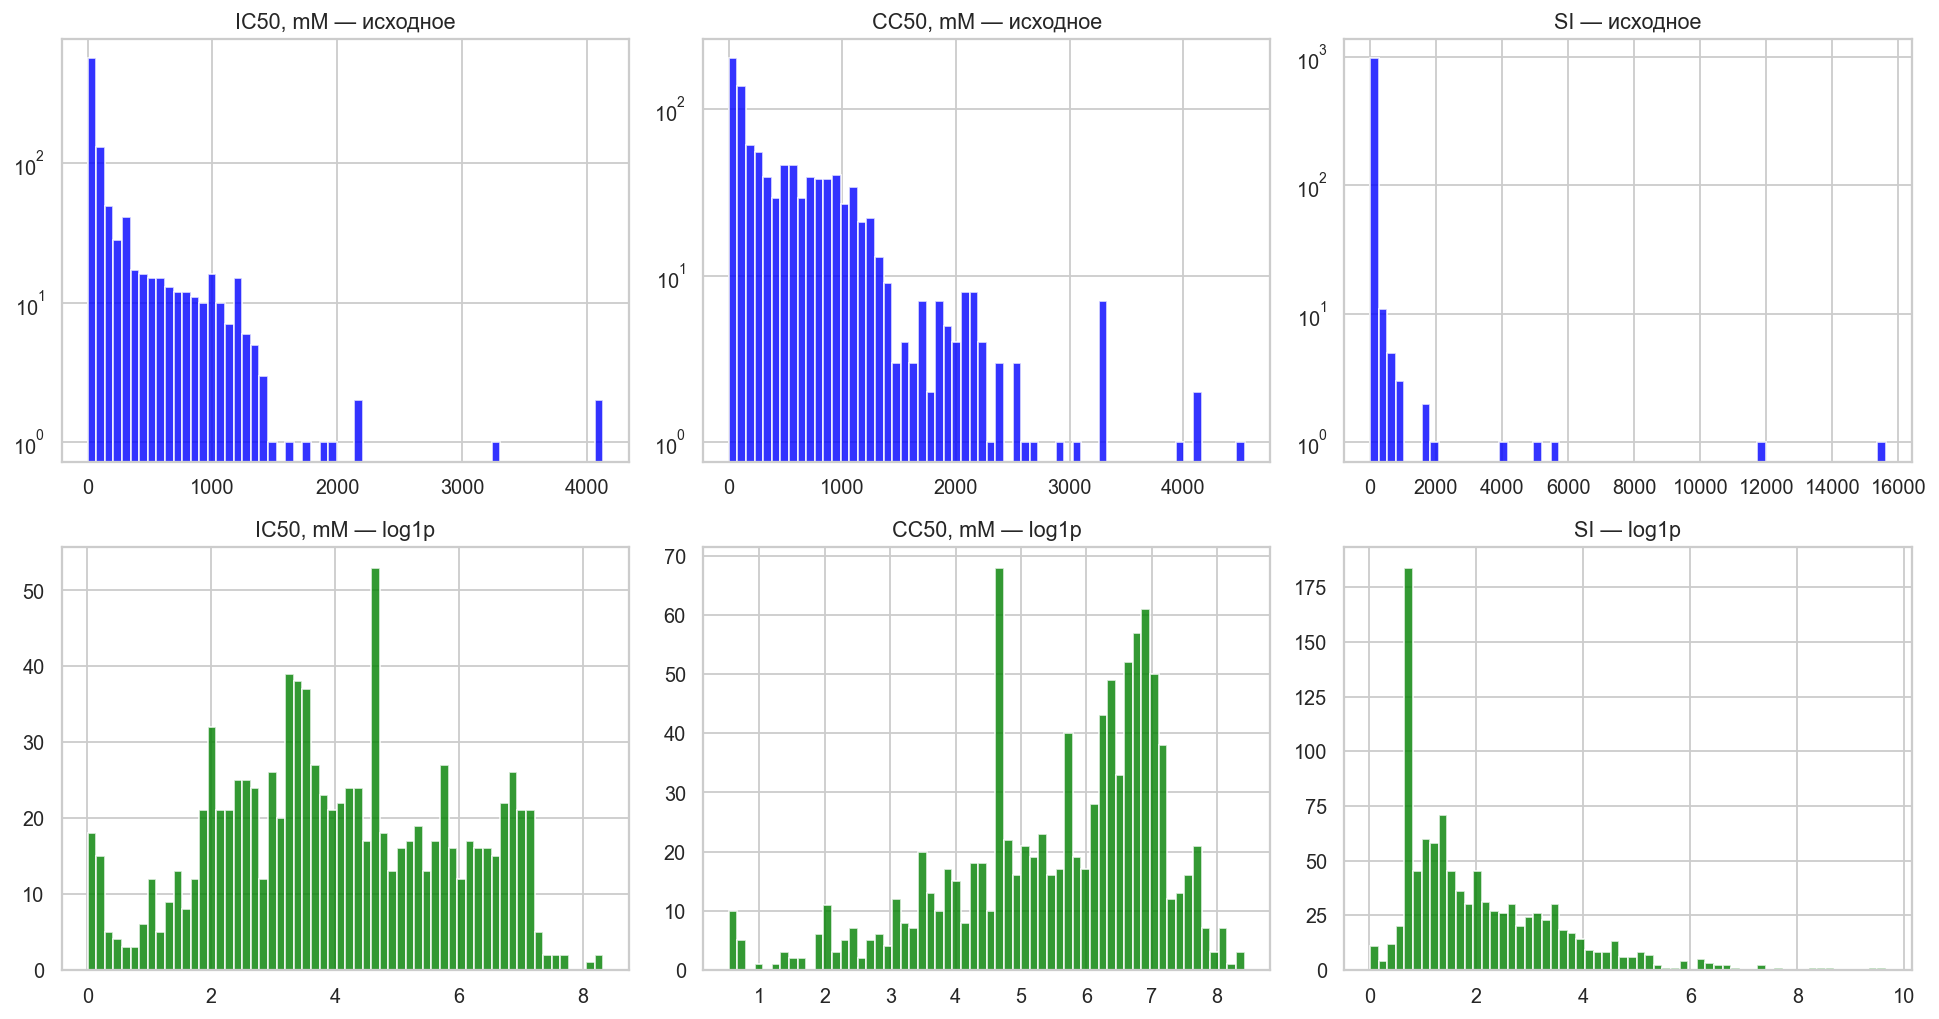
\includegraphics[width=\textwidth]{figures/01_target_distributions.png}
    \caption{распределения целевых до и после преобразования лог1п }
    \label{fig:target_dist}
\end{figure}

Боксплоты подтверждают наличие большого количества выбросов - особенно для SI.

\begin{figure}[H]
    \centering
    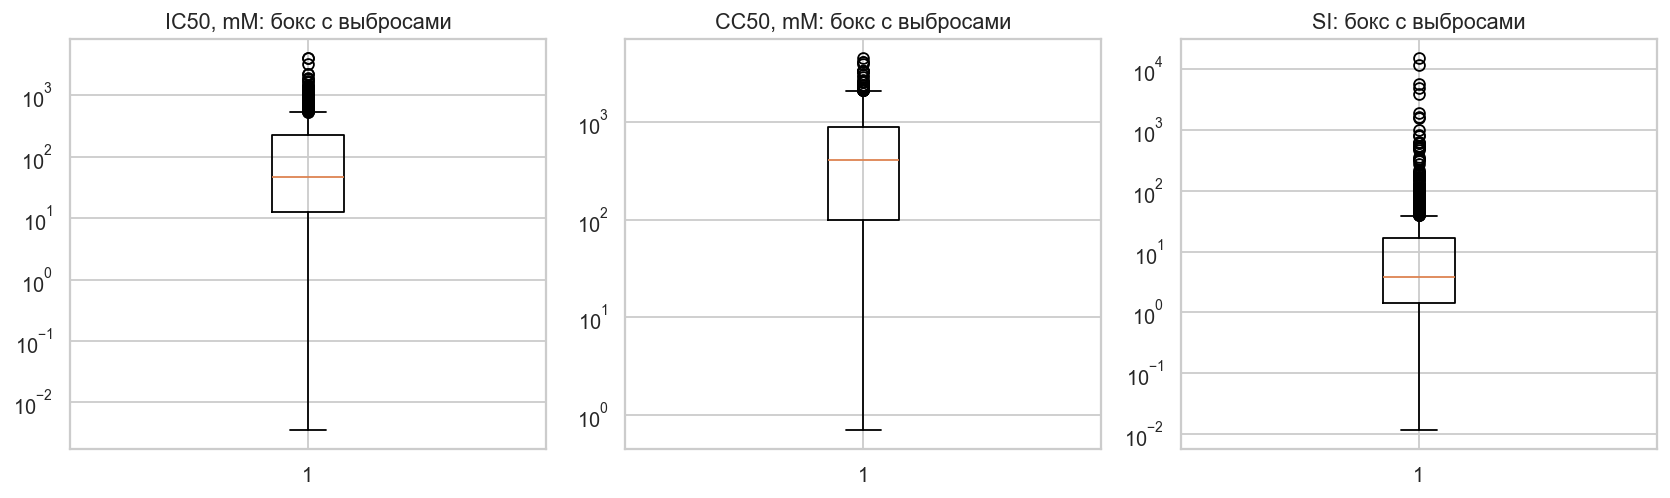
\includegraphics[width=\textwidth]{figures/02_target_boxplots.png}
    \caption{боксплоты целевых переменных}
    \label{fig:boxplots}
\end{figure}

Вывод: для регрессионных задач решено обучать на логарифмированных целевых переменных - это стабилизирует обучение, особенно для линейных моделей и снижает влияние единичных выбросов на функцию потерь. Ещё для регрессионных применяется фильтрация выбросов по правилу 3*IQR. 

\section{Парные зависимости между таргетами}

На парных графиках видно, что IC50 и CC50 связаны умеренно (чисто визуально - при большем значении одной переменной - в среднем больше и другой. И vice versa). 

Формула SI=CC50/IC50, но по pairplot, само отношение не видно - только отдельные пары. Корреляция SI с IC50 - прослеживается хорошо. С СС50 - слабее.

\begin{figure}[H]
    \centering
    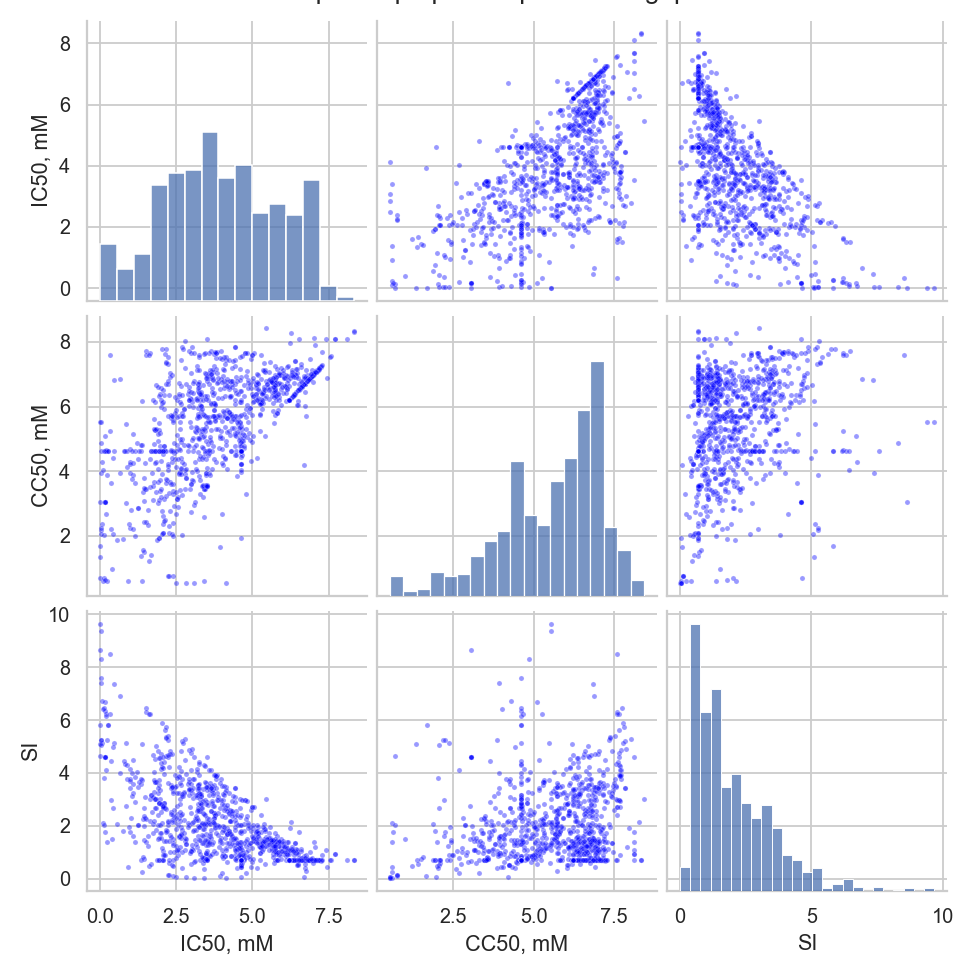
\includegraphics[width=0.95\textwidth]{figures/03_targets_pairplot.png}
    \caption{парные графики}
    \label{fig:pairplot}
\end{figure}

Вывод. Умеренная связь IC50 и CC50 при зависимости SI от обоих парметров, говорит о том что задача регрессии SI всё-таки сложнее - ошибки прогнозов базовых таргетов перемножаются в производной величине.

\section{Корреляционный анализ признаков с таргетами}

Построена тепловая карта, для 30 признаков с наибольшей корреляцией хотя бы с одним из таргетов. Макс значение корреляции одного признака с одним таргетом не превышает 0.27 (например, NumSaturatedHeterocycles для IC50, Kappa3 для CC50, FractionCSP3 для SI) значит ни один из признаков в одиночку не объясняет целевую в значимой мере.

\begin{figure}[H]
    \centering
    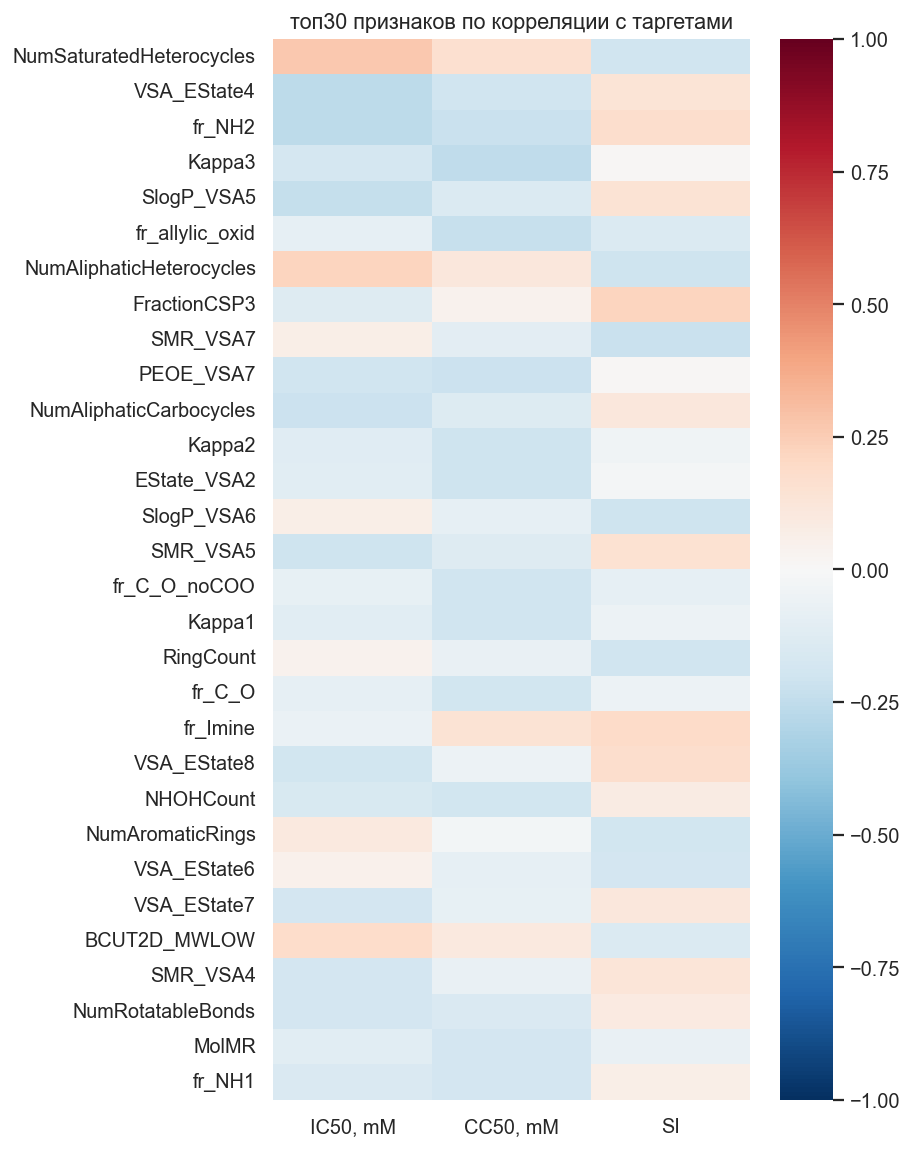
\includegraphics[width=0.7\textwidth]{figures/04_top_corr_with_targets.png}
    \caption{Тепловая карта корреляций топ30 признаков с целевыми переменными}
    \label{fig:corr}
\end{figure}

Вывод:связь признаков с таргетами нелинейная; это означает что качества стоит ожидать от моделей ансамблей на решающих деревьях - Random Forest, XGBoost~\cite{habr-xgboost} и LightGBM - они умеют ловить нелинейности и взаимодействия признаков. Линейные - Ridge, ElasticNet по сути бесполезны и добавлены как минимальный порог качества (просто увидеть, насколько ансамбли лучше)

(по факту так и получилось: во всех 7 задачах, "победили" деревья)


\section{Фильтрация признаков}

В предобработке реализовано:
\begin{itemize}
    \item удаление пропущенных колонок;
    \item удаление колонок с низкой дисперсией - константы (по ЕДА - 18);
    \item удаление одного из членов каждой пары с |p| > 0.95 (по ЕДА - 33).
\end{itemize}

Результаты EDA: всего: пустых колонок --- 0, констант --- 18, скоррелированных --- 33. В результате остаётся 159 признаков. В пайплайне моделей фильтрация повторяется после удаления выбросов по таргету, поэтому число оставшихся признаков для разных задач чуть колеблется (157-159).

Вывод: удаление мусорных и избыточных признаков ускоряет обучение и стабилизирует линейные модели. 

\section{Баланс классов для задач классификации}

Распределение положительного класса для четырёх классификационных задач показано на рисунке 3.5. Для задач "выше медианы" доля положительного класса близка к 50\% по построению. Задача SI>8 имеет умеренный дисбаланс (35.7\% положительных).

\begin{figure}[H]
    \centering
    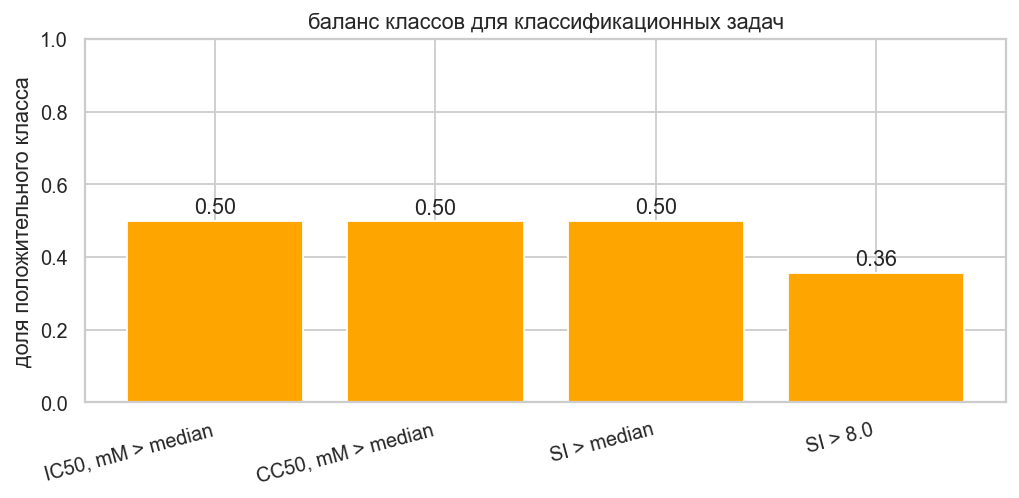
\includegraphics[width=0.85\textwidth]{figures/05_class_balance.png}
    \caption{Доля положительного класса для четырёх задач классификации}
    \label{fig:class_balance}
\end{figure}

\textbf{Вывод.} Для  \texttt{SI>8} необходимо учитывать дисбаланс классов: в моделях, поддерживающих параметр \texttt{class\_weight='balanced'} (лог.регр, случ.лес, лгбм) - он включён, для XGBoost используется параметр \texttt{scale\_pos\_weight}, равный отношению числа отрицательных примеров к положительным. В качестве целевой метрики для подбора гиперпараметров во всех классификационных задачах выбран roc-auc -  показатель качества бинарного классификатора, который оценивает, как хорошо модель умеет отделять положительный класс от отрицательного при любом пороге; 0.5 - это типа угадывания, 1.0 - идеальное разделение. Эта метрика слабо чувствительна к дисбалансу классов, поэтому удобна для всех 4х задач.

\section{Область применимости (Applicability Domain)}

Для оценки области применимости моделей рассчитан стандартизованный leverage --- ср.кв z-нормированных значений признаков для каждого объекта. Среднее по выборке - 1.00, leverage\_p95 --- 2.43 , 49 соединений за этим пределом (т.е. 49/1001 == примерно 4.9\% выборки).

\textbf{Вывод.} Предсказания моделей для соединений, попадающих в эту группу --- можно считать "ненадёжными".
\section{Сводка решений по EDA}

По результатам EDA приняты следующие проектные решения, применяемые во всех семи моделях:
\begin{enumerate}
    \item для регрессий целевая переменная преобразуется как log(1+y);
    \item для регрессий применяется фильтрация выбросов по правилу 3*IQR от таргета;
    \item признаковое пространство фильтруется (константы, |p|>0.95, NaN-колонки), оставшиеся пропуски импутируются медианой;
    \item для классификационных задач применяется стратифицированный split, а для задачи \texttt{SI > 8} дополнительно используются веса классов;
    \item в качестве линии сравнения включены как линейные, так и древесные модели, чтобы количественно подтвердить нелинейность задачи.
\end{enumerate}

% ===========ИНСТРУМЕНАТРИЙ ====================
\chapter{Инструментарий и методология моделирования}

\section{Использованные библиотеки}

В работе использовался Python 3.11 и следующие библиотеки: \texttt{pandas} и \texttt{numpy} , \texttt{scikit-learn} ; \texttt{xgboost} и \texttt{lightgbm} --- специализированные реализации градиентного бустинга (XGBoost, особенности и параметры в~\cite{habr-xgboost}); \texttt{optuna} для подбора гиперпараметров через Tree Parzen Estimator ~\cite{habr-optuna}; \texttt{matplotlib} и \texttt{seaborn}, \texttt{joblib} для сериализации. Управление окружением осуществляется через менеджер пакетов \texttt{uv} с фиксацией версий в \texttt{uv.lock}.

\section{Состав моделей-кандидатов}

Выбор моделей обоснован конспектом и расширен градиентным бустингом (3 модели) для сравнения. Для регрессионных задач протестировано семь моделей-кандидатов, для классификационных --- шесть. Полный перечень :

\begin{table}[H]
\centering
\caption{Модели}
\label{tab:models}
\begin{tabular}{lll}
\toprule
Модель & Регрессия & Классификация \\
\midrule
Ridge / Logistic Regression          & \checkmark Ridge        & \checkmark LogReg \\
ElasticNet                            & \checkmark              & --- \\
K-Nearest Neighbors                   & \checkmark              & \checkmark \\
Random Forest                         & \checkmark              & \checkmark \\
Gradient Boosting (sklearn)           & \checkmark              & \checkmark \\
XGBoost                               & \checkmark              & \checkmark \\
LightGBM                              & \checkmark              & \checkmark \\
\bottomrule
\end{tabular}
\end{table}

Линейные и KNN требуют масштабирования признаков, поэтому собираются через \texttt{sklearn.pipeline.Pipeline} с \texttt{StandardScaler}. 

Все модели с поддержкой балансировки получают параметр \texttt{class\_weight='balanced'}, для XGBoost дополнительно вычисляется \texttt{scale\_pos\_weight} в задаче с дисбалансом.

\section{Единый пайплайн обучения}

Все семь задач идут по одному алгоритму в методе \texttt{run()} абстрактного \texttt{BaseTask}. 

Шаги пайплайна:
\begin{enumerate}
    \item загрузка через \texttt{data\_io.load\_raw};
    \item фильтрация признаков (\texttt{preprocessing.filter\_features}), удаление выбросов по таргету (регрессии), заполнение пропусков медианой, преобразование целевой переменной (\texttt{log1p} для регрессий, бинаризация для классификаций);
    \item разделение на обучающую и отложенную выборки - 80/20 (для классификаций --- стратифицированное по таргету);
    \item для каждой модели-кандидата --- запуск Optuna: 40, TPE с фиксированным random=42; внутри каждого испытания 5-кратная кросс-валидация на обучающей выборке;
    \item дообучение лучшей конфигурации каждой модели на полной обучающей выборке и оценка на отложенной;
    \item выбор победителя по средней метрике кросс-валидации; сохранение всех артефактов задачи в \texttt{artifacts/}.
\end{enumerate}

В качестве метрики для подбора гиперпараметров используется \texttt{neg\_root\_mean\_squared\_error} для регрессии и \texttt{roc\_auc} для классификации. Финальная оценка проводится по: MAE, RMSE, R\^{}2 для регрессии; accuracy, precision, recall, F1, ROC-AUC для классификации.

% ================РЕЗ РЕГРЕССИЙ ====================
\chapter{Результаты регрессионных моделей}

Сводка по всем регрессионным задачам: 
\begin{table}[H]
\centering
\caption{Результаты регрессионных моделей}
\label{tab:reg_summary}
\begin{tabular}{lllrrr}
\toprule
Задача & Таргет & Лучшая модель & MAE (log) & RMSE (log) & R\^{}2 \\
\midrule
regression\_ic50 & IC50 & XGBoost        & 1.016 & 1.282 & 0.416 \\
regression\_cc50 & CC50 & Random Forest  & 0.805 & 1.087 & 0.511 \\
regression\_si   & SI   & Random Forest  & 0.745 & 0.932 & 0.171 \\
\bottomrule
\end{tabular}
\end{table}

\section{Регрессия IC50}

Лучшей моделью по итогам кросс-валидации стала \textbf{XGBoost}. Гиперпараметры: \texttt{n\_estimators=256}, \texttt{learning\_rate=0.023}, \texttt{max\_depth=4}, \texttt{subsample=0.66}, \texttt{colsample\_bytree=0.82}, \texttt{reg\_lambda=9.19}. На отложенной выборке достигнуты: MAE=1.016, RMSE=1.28, R\^{}2=0.416.   

Линейные модели (Ridge, ElasticNet) показали отрицательный R\^{}2  т.е. фактически оказались хуже чем предсказания средним значением.  Ансамбли (Random Forest, GradientBoosting, XGBoost, LightGBM) уверенно решают задачу с R\^{}2 - 0.34--0.42, но в лидерах XGBoost+RF+GB. LGBM - 0.34

\textbf{Вывод и рекомендации.} Достигнутое качество достаточно для предварительного отобора кандидатов. Возможные улучшения: построение отдельной модели "активен/неактивен" для подвыборки сверхактивных соединений с последующей регрессией внутри подвыборки, ну и конечно стэкинг лучших ансамблевых моделей.

\section{Регрессия CC50}

Лучшая модель -- \textbf{Random Forest} с конфигом: \texttt{n\_estimators=660}, \texttt{max\_depth=23}, \texttt{min\_samples\_split=7}, \texttt{min\_samples\_leaf=2}, \texttt{max\_features='sqrt'}. Метрики на отложенной выборке: MAE=0.81, RMSE=1.09, R\^{}2=0.511.

Регрессия сс50 оказалась самой предсказуемой из трёх регрессионных задач. Все ансамблевые модели показали близкое качество (R\^{}2 в диапазоне 0.49--0.53), линейные модели конечно хуже - R\^{}2 около 0.28-0.32, но всё равно - положительный R\^{}2. 

Вывод и рекомендации: Модель СС50 - самая надёжная из трёх и может использоваться как первичный фильтр.

\section{Регрессия SI}

Лучшая модель опять \textbf{Random Forest} (\texttt{n\_estimators=528}, \texttt{max\_depth=16}, \texttt{min\_samples\_split=7}, \texttt{min\_samples\_leaf=4}, \texttt{max\_features='log2'}). Метрики: MAE=0.74, RMSE=0.93, R\^{}2=0.171.

Результат слабее остальных регрессий: SI является производной от IC50 и CC50 и ошибки исходных таргетов при делении \emph{ накапливаются}. Этот гипотеза из EDA, полностью подтверждена  количественно: даже лучшая модель объясняет лишь около 17\% дисперсии log(1+si). Все ансамбли показали близкое качество - R\^{}2 около 0.13--0.17, линейные --- около R\^{}2 0.07--0.08.

\textbf{Вывод и рекомендации.} Прямую регрессию si использовать только как контрольный бейзлайн. В практических задачах si получать только как pred(CC50) / pred(IC50) из предсказаний двух более точных.

% ======= РЕЗУЛЬТ. КЛАССИФ==========
\chapter{Результаты классификационных моделей}

Сводка по всем классификационным задачам приведена в табл.~\ref{tab:clf_summary}. Основная метрика - ROC-AUC. Доп: accuracy, precision, recall, F1.

\begin{table}[H]
\centering
\caption{Результаты классификационных моделей }
\label{tab:clf_summary}
\small
\begin{tabular}{lllrrrrr}
\toprule
Задача & Таргет & Лучшая модель & Accuracy & Precision & Recall & F1 & ROC-AUC \\
\midrule
classification\_ic50\_median & IC50 > med   & Random Forest    & 0.711 & 0.675 & 0.81 & 0.736 & 0.779 \\
classification\_cc50\_median & CC50 > med   & GradientBoosting & 0.716 & 0.684 & 0.8 & 0.737 & 0.832 \\
classification\_si\_median   & SI > med     & Random Forest    & 0.657 & 0.687 & 0.57 & 0.623 & 0.704 \\
classification\_si\_gt8      & SI > 8       & XGBoost          & 0.731 & 0.667 & 0.5 & 0.571 & 0.744 \\
\bottomrule
\end{tabular}
\end{table}

\section{Классификация: IC50 выше медианы}

Лучшей моделью стала \textbf{Random Forest}. На отложенной выборке достигнут ROC-AUC=0.779, F1=0.736. Из шести кандидатов четыре - ансамблевые модели на решающих деревьях (Random Forest, GradientBoosting, XGBoost, LightGBM) показали ROC-AUC - 0.76--0.78, то есть результат устойчив к выбору конкретного ансамбля. Лог. регрессия даёт чуть меньше (около 0.75), но сопоставимый F1 - задача выше/ниже медианы в целом нормально разделяется даже простой линейной моделью.

\textbf{Вывод.} Модель хорошо отделяет два класса: auc - 0.779, f1 - 0.736. Это подтверждает что бинаризация по медиане ИС50 - адекватная задача для табличных моделей.

\section{Классификация: CC50 выше медианы}

Лучший результат - \textbf{GradientBoosting}: ROC-AUC=0.832, F1=0.737. Это самая удачная из четырёх классификаций: метрики выше остальных, модели ведут себя стабильно.

\textbf{Вывод.} Для бинаризации CC50 по медиане - GradientBoosting - лучший выбор. Имеет смысл смотреть вместе с регрессией CC50: если регрессия и классификация расходятся, объект стоит проверить отдельно.

\section{Классификация: SI выше медианы}

Лучшей моделью стала \textbf{Random Forest} с ROC-AUC=0.704 и F1=0.623. Но как и в регрессии - это самая слабая классификация из четырёх. Причина та же: SI считается из IC50 и CC50, поэтому связь с признаками менее прямая, чем у отдельных таргетов.

\textbf{Вывод.} Отдельная классификация SI по медиане даёт скромный результат. 

\section{Классификация: SI > 8}

Лучшая модель --- \textbf{XGBoost} с гиперпараметрами \texttt{n\_estimators=419}, \texttt{learning\_rate=0.015}, \texttt{max\_depth=9}, \texttt{subsample=0.71}, \texttt{colsample\_bytree=0.78}, \texttt{reg\_lambda=9.21}. Метрики на отложенной выборке: ROC-AUC=0.744, accuracy=0.731, precision=0.667, recall=0.500, F1=0.571.

Здесь умеренный дисбаланс (35.7\% c si>8), порог задан в условии. 

Ансамбли дают ROC-AUC около 0.73--0.76, но recall ниже (0.47--0.58): признаки "на границе", модель чаще относит классу большинства - типа как "безопасный" прогноз. Как аналогия: в~\cite{habr-mit-antibiotics} похожий приём --- ML-скрининг на большой выборке с последующей ручной проверкой лучших кандидатов (только там размер выборки - 12 076 365 соединений) .

\textbf{Вывод и рекомендации.} Модель рабочая, но recall слабый. Можно снизить порог вероятности с 0.5 до около 0.3 и попробовать добавить \texttt{CalibratedClassifierCV} для калибровки~\cite{habr-mlbootcamp}, если важнее поймать больше положительных примеров.

% ========= АНАЛИЗ+ОБСУЖДЕНИЕ ===
\chapter{Сравнительный анализ и обсуждение}

\section{Регрессия против классификации}

Чисто по метрикам, классификации в среднем выглядят сильнее регрессий, что и логично: предсказывать выше/ниже порога -- проще, чем предсказывать точное число. Если нужен только отсев или ранжирование по половинам выборки --- классификация. Если нужно именно значение таргета -- регрессия.

\section{Линейные модели против ансамблей}

Во всех семи задачах древесные ансамбли (Random Forest, XGBoost, GradientBoosting и даже "слабый" LightGBM) явно превосходят линейные модели по основной метрике (что собственно и говорилось ещё в EDA). Особенно это проявилось в регрессии IC50, где линейные не смогли превзойти даже предсказание средним. Это согласуется с EDA: ни один из 210 признаков по отдельности, таргет почти не объясняет (|p|\_max около 0.27),  связь скорее нелинейная, соответственно выбор древесных - вполне логичен.

\section{Согласованность EDA и финальных результатов}

Решения по EDA нашли отражение в метриках:
\begin{itemize}
    \item \emph{Преобразование log(1+y)} -- без него линейные модели не работают от слова совсем (отрицательный R\^{}2 даже после логарифмирования, без логарифмирования - ещё хуже из-за выбросов)
    \item \emph{Удаление коррелированных признаков} - качество не просело после сокращения с 210 до 157-159 признаков, обучение стало быстрее
    \item \emph{Производный характер SI} -- регрессия SI явно слабее CC50 и IC50 что и ожидалось
    \item \emph{Дисбаланс в задаче \texttt{SI > 8}} -- precision выше recall, типично для дисбаланса даже с весами классов
    \item \emph{Ансамбли на деревьях} -- победили во всех 7 задачах по основной метрике
\end{itemize}

\section{Нюансы}

\begin{itemize}
    \item Чуть меньше 5\% объектов выбиваются по leverage -- для них предсказания менее надёжны
    \item Регрессия SI по факту дублирует IC50 и CC50: в задании она есть, но лучше считать SI из двух более сильных регрессий
    \item 1001 строка -- не очень много для тяжёлых моделей. На большем датасете, качество скорее всего бы выросло
\end{itemize}

\section{Рекомендации по развитию}

\begin{enumerate}
    \item Для \texttt{SI>8} -- \texttt{CalibratedClassifierCV} и подбор порога под нужный баланс precision/recall
    \item Стэкинг RF+XGBoost+LightGBM по predict на holdout, где несколько моделей близки по метрике
    \item SHAP для лучших моделей RF, XGBoost, LightGBM. В работе не пробовал, но судя обзору~\cite{habr-shap-lime} для таких моделей есть Tree SHAP, который покажет вклад каждого из 210 дескрипторов в конкретное предсказание и summary plot (что-то типа картинки важности признаков по всей выборке) по отложенной выборке. Dependence plot показал бы взаимодействия между X и Y - типа графика как при значении признака реагирует модель. И что-то типа "правдоподобности правил модели" - на какие дескрипторы модель опирается и нет ли подозрительных признаков (утечки). Авторы пишут, что при сильной корреляции дескрипторов вклад "размазываеться" между признаками. В целом, судя по статье, это именно тот инструментарий, который помог бы разобраться с обученными моделями и понять какие дескрипторы реально "тянут" предсказание 
\end{enumerate}

% ========= ИИИИ... ЗАКОНЧИЛИ!  ====================
\chapter*{Заключение}
\addcontentsline{toc}{chapter}{Заключение}

В рамках курсовой выполнен полный ML-пайплайн на табличном датасете:

\begin{itemize}
    \item разобран учебный материал (конспект студентов, статьи на Хабре) по классическому МО и подбору гиперпараметров
    \item сделаны EDA и предобработка: log1p для регрессий, фильтрация признаков, 3*IQR, стратификация, веса классов для \texttt{SI > 8}
    \item сравнено 6-7 моделей на задачу, Optuna(TPE, 5fold, 40trials)
    \item итоговые метрики по тестовой части: лучшие R\^{}2 --- CC50 0.51 (RF), IC50 0.42 (XGBoost), SI 0.17 (RF), классификации ROC-AUC 0.70--0.83
    \item даны рекомендации как можно улучшить, если взяться за задучу всерьёз (калибровка, стэкинг, SHAP)
    \item собрано Python-приложение: src-layout,pyproject.toml, "растовский" uv, единый пайплайн на семь задач, логирование. Хоть где-то можно пилить, как хочешь и реализовывать "красивую" архитектуру, а не "абы-как, лишь бы было сделано вчера, а заказчику - прокатит, что-нибудь придумаем".
    \item написан отчёт в TexShop на движке XeLaTex:) и вряд ли кто-то до сюда дочитает, поэтому можно откровенно признаться: я "заманался" с этим заданием.
\end{itemize}

Полный исходный код, данные, графики EDA, модели и метрики - в репозитории: 

\url{https://github.com/stepkar/chemical-coursework}.

% ==== ЛИТЕРКАТУРА ==========
\begin{thebibliography}{9}


\bibitem{cc50-ic50}
\textbf{Creative Diagnostics.}
CC50/IC50 Assay for Antiviral Research. ---
Электронный ресурс:
\url{https://antiviral.creative-diagnostics.com/cc50-ic50-assay.html}.


\bibitem{lectures-msu}
\textbf{TeachInMSU.}
ИСКУССТВЕННЫЙ ИНТЕЛЛЕКТ В ХИМИИ И МАТЕРИАЛОВЕДЕНИИ (МИТРОФАНОВ АРТЕМ АЛЕКСАНДРОВИЧ и др.: конспект курса лекций.)
Химфак МГУ

\bibitem{fluent-python}
\textbf{Luciano Ramalho}
Fluent Python: Clear, Concise, and Effective Programming. ---
2nd edition --- O'Reilly, 2022.

\bibitem{habr-optuna}
\textbf{badcasedaily1.}
Библиотека Optuna в Python для оптимизации гиперпараметров. ---
Хабр, блог компании OTUS, 2024. ---
\url{https://habr.com/ru/companies/otus/articles/801463/}.

\bibitem{habr-xgboost}
\textbf{XGBoost: особенности работы.} ---
Хабр, 2024. ---
\url{https://habr.com/ru/articles/799725/}.

\bibitem{habr-sklearn}
\textbf{Гайд по Scikit-learn в 2025: собираем пайплайн, который не сломается.} ---
Хабр, блог компании Нетология, 2025. ---
\url{https://habr.com/ru/companies/netologyru/articles/911216/}.

\bibitem{habr-mit-antibiotics}
\textbf{ИИ помог обойти защиту резистентных бактерий: открыт новый класс перспективных антибиотиков.} ---
Хабр, блог компании BotHub, 2024. ---
\url{https://habr.com/ru/companies/bothub/articles/788170/}.

\bibitem{habr-mlbootcamp}
\textbf{m0rtido.}
Варим ML Boot Camp III: Starter Kit. ---
Хабр, 2017. ---
\url{https://habr.com/ru/articles/324924/}.

\bibitem{habr-shap-lime}
\textbf{boygenius13.}
Интерпретация моделей и диагностика сдвига данных: LIME, SHAP и Shapley Flow. ---
Хабр, блог компании Open Data Science, 2022. ---
\url{https://habr.com/ru/companies/ods/articles/599573/}.

\end{thebibliography}

\end{document}